\documentclass[a4paper,12pt]{article}
\usepackage[utf8]{inputenc}
\usepackage[russian]{babel}
\usepackage[OT1]{fontenc}
\usepackage{amsmath}
\usepackage{amsfonts}
\usepackage{amssymb}
\usepackage{graphicx}
\graphicspath{{Images/}}
\usepackage[left=2cm,right=2cm,top=2cm,bottom=2cm]{geometry}
\usepackage{calc}
\usepackage{wrapfig}
\usepackage{setspace}
\usepackage{indentfirst}
\usepackage{subfigure}

% Математика
\usepackage{amsmath,amsfonts,amssymb,amsthm,mathtools}


\usepackage{wasysym}

%Заговолок
\author{Талашкевич Даниил Александрович}

\title{Лабораторная работа 1.2.5}

\date{\today}

\begin{document}

\maketitle
\thispagestyle{empty}

\newpage
\setcounter{page}{1}

	\textbf{Цель работы:} исследовать вынужденную прецессию гироскопа; установить зависимость скорости вынужденной прецессии гироскопа от величины момента сил, действующих на ось гироскопа; определить скорость вращения ротора гироскопа и сравнить ее со скоростью, рассчитанной по скорости прецессии.
	
	\textbf{В работе используются:} гироскоп в кардановом подвесе, секундомер, набор грузов, отдельный ротор гироскопа, цилиндр известной массы, крутильный маятник, штангенциркуль, линейка. 


\section{Теоретический материал.}

Основные уравнения движения твердого тела можно записать в виде:

\begin{equation}
	\frac{d\vec{P}}{dt} = \vec{F}
	\label{eq:center_of_mass}
\end{equation}

\begin{equation}
	\frac{d\vec{L}}{dt} = \vec{M}
	\label{eq:moments_equation}
\end{equation}

Формула (\ref{eq:center_of_mass}) выражает закон движения центра масс, а формула (\ref{eq:moments_equation}) -- уравнение моментов, действующих на тело. Двух данных уравнений достаточно для описания состояния твердого тела.

Если сила $\vec{F}$ не зависит от угловой скорости вращения тела, а момент $\vec{M}$ от скорости поступательного движения тела, то уравнения (\ref{eq:center_of_mass}) и (\ref{eq:moments_equation}) можно рассматривать независимо друг от друга. В данной работе рассматривается только задача о вращении твердого тела.

Момент импульса твердого тела можно вычислить, используя формулу:
\begin{equation}
	\vec{L} = \vec{i}I_{x}\omega_{x} + \vec{j}I_{y}\omega_{y} + \vec{k}I_{z}\omega_{z},
\end{equation}
где $ I_{x},I_{y},I_{z} $ -- главные моменты инерции тела, $ \omega_{x}, \omega_{y}, \omega_{z} $ -- компоненты вектора угловой скорости  $\vec{\omega} $.

Быстро вращающееся тело, для которого:

	$$I_{z}\omega_{z} \gg I_{x}\omega_{x}, I_{y}\omega_{y}$$

принято называть \textit{гироскопом}. Гироскоп называется уравновешенным, если его центр масс неподвижен.

В силу (\ref{eq:moments_equation}), приращение момента импулься определяется интегралом:
\begin{equation}
	\Delta\vec{L} =  \int\vec{M}\\,dt
	\label{eq:integral_for_increment}
\end{equation}

Если момент внешних сил действует в течение короткого промежутка времени, из формулы (\ref{eq:integral_for_increment}) следует, что приращение $\vec{L}$ момента импулься значительно меньше самого момента импульса, т.е:

\begin{equation}
	\left| \Delta\vec{L} \right| \ll \left| \vec{L} \right|.
\end{equation}

Благодаря этому, гироскоп приобретает очень большую устойчивость, вызванную его быстрым вращением.

Если гироскоп уравновешен, то суммарный момент сил, действующих на него, равен 0. В таком случае, гироскоп не будет изменять своего положения в пространстве. Если на гироскоп в течение длительного времени будет действовать некоторый момент сил, отличный от нуля, то, согласно (\ref{eq:moments_equation}) гироскоп придет в движение. Мы не будем рассматривать действие моментов сил, которые вызовут ускорение или замедление гироскопа (т.е. моментов сил, которые не изменяют положения оси вращения гироскопа). Рассмотрим действия моментов сил, которые изменяют положение оси вращения гироскопа.

\begin{wrapfigure}[19]{r}{0.4\textwidth}
	\vspace{-2.5ex}
	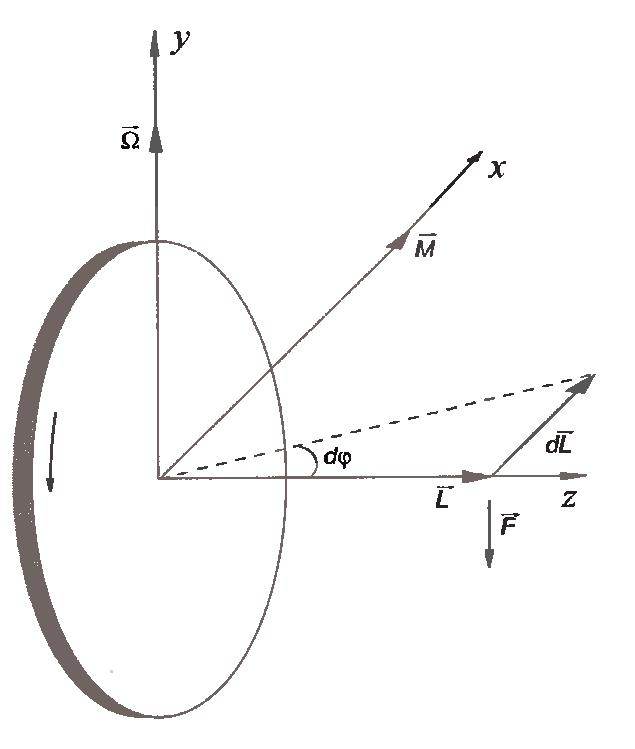
\includegraphics[width = 0.35\textwidth]{flywheel}
	\caption{Маховик.}
	\label{fig:flywheel}
\end{wrapfigure}

Рассмотрим маховик, вращающийся вокруг оси z. (Рис. \ref{fig:flywheel}). Будем считать, что 
$$ \omega_{z} = \omega_{0},\qquad \omega_{x} = \omega_{y} = 0.$$

Пусть ось вращения повернулась в плоскости \textit{zx} по направлению в оси \textit{x} на бесконечно малый угол $d\varphi$. Такой поворот означает добавочное вращение маховика вокруг оси \textit{y}, так что 
$$ d\varphi = \Omega\,dt, $$
где $ \Omega $ -- угловая скорость такого вращения. Будем предполагать, что
\begin{equation}
	L_{\Omega} \ll L_{\omega_{0}}
	\label{eq:condition_for_rotate}
\end{equation}

Это означает, что момент импульса маховика, равный $I_{z}\omega_{0}$ до приложения внешних сил, только повернется в плоскости \textit{zx} по направлению к оси \textit{x} не изменяя своей величины. Таким образом,

\begin{equation}
	\left|d\vec{L}\right| = Ld\varphi = I\Omega\,dt
	\label{eq:increment_moment_of_impulse}
\end{equation}


Записывая выражение (\ref{eq:increment_moment_of_impulse}) в виде векторного произведения, получаем:

\begin{equation}
	\frac{d\vec{L}}{dt} = \vec{\Omega} \times \vec{L}
\end{equation}

Окончательно, используя (\ref{eq:moments_equation}), получаем:

\begin{equation}
	\vec{M} = \vec{\Omega} \times \vec{L}
	\label{eq:rotation_by_moments_of_force}
\end{equation}

Формула (\ref{eq:rotation_by_moments_of_force}) справедлива, если выполнено условие (\ref{eq:condition_for_rotate}).
Данная формула позволяет определить, момент сил $ \vec{M}, $ который нужно приложить к маховику, чтобы вызвать вращение маховика с угловой скоростью $\vec{\Omega}$.

Под действием момента внешних сил $\vec{M}$ ось гироскопа медленно вращается вокруг оси \textit{y} с угловой скоростью $\vec{\Omega}$. Такое движение называют \textit{прецессией гироскопа}.

Для изучения регулярной прецессии уравновешенного гироскопа к его оси подвешивают дополнительные грузы. Это смещает общий центр масс и создает момент сил тяжести, вызывающий прецессию. Скорость прецессии в этом случае может быть найдена по формуле:

\begin{equation}
	\Omega = \frac{mgl}{I_{z}\omega_{0}},
	\label{eq:teor_equation_omega}
\end{equation} 
где m -- масса груза, l -- расстояние от центра карданова подвеса до точки крепления груза на оси гироскопа. (Рис. \ref{fig:facility})

Для выполнения работы используется гироскоп (Рис. \ref{fig:facility}), закрепленный в карданном подвесе (Рис. \ref{fig:Cardan_suspension}).


\begin{figure}[ht!]  
	\vspace{-4ex} 
	\centering 
	\subfigure[]{
		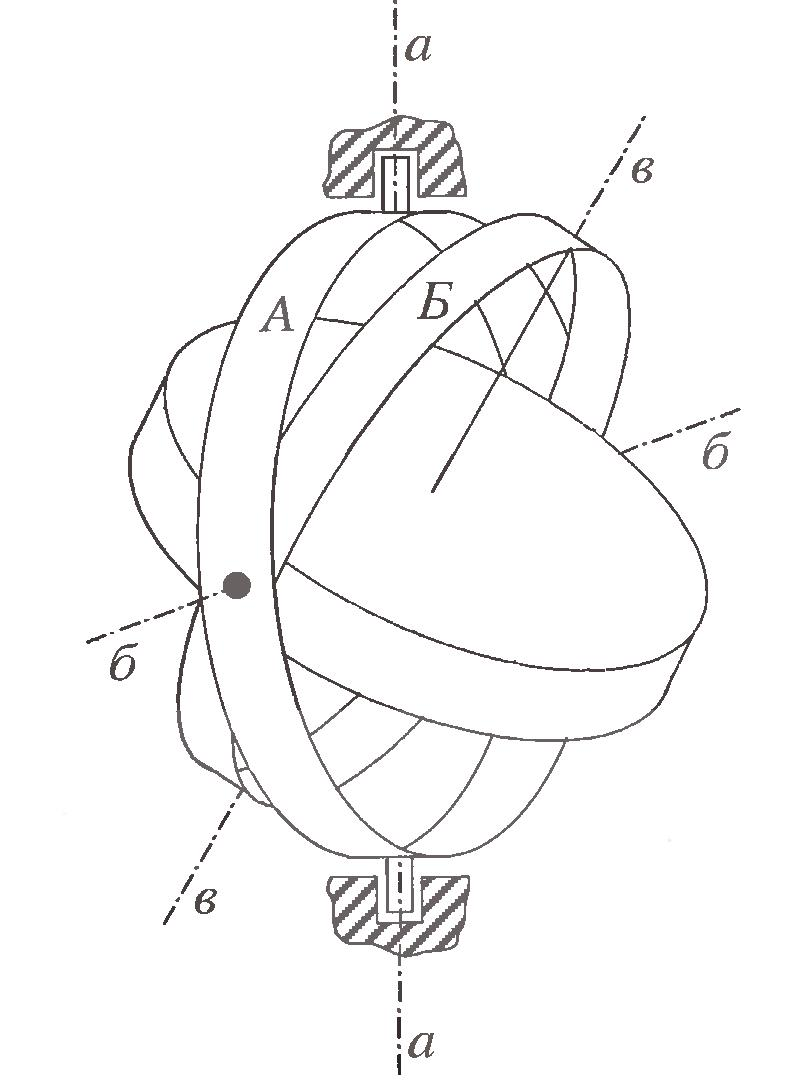
\includegraphics[width=0.29\linewidth]{Cardan_suspension} 	
			\label{fig:Cardan_suspension}}  
	\hspace{4ex}
	\subfigure[]{
		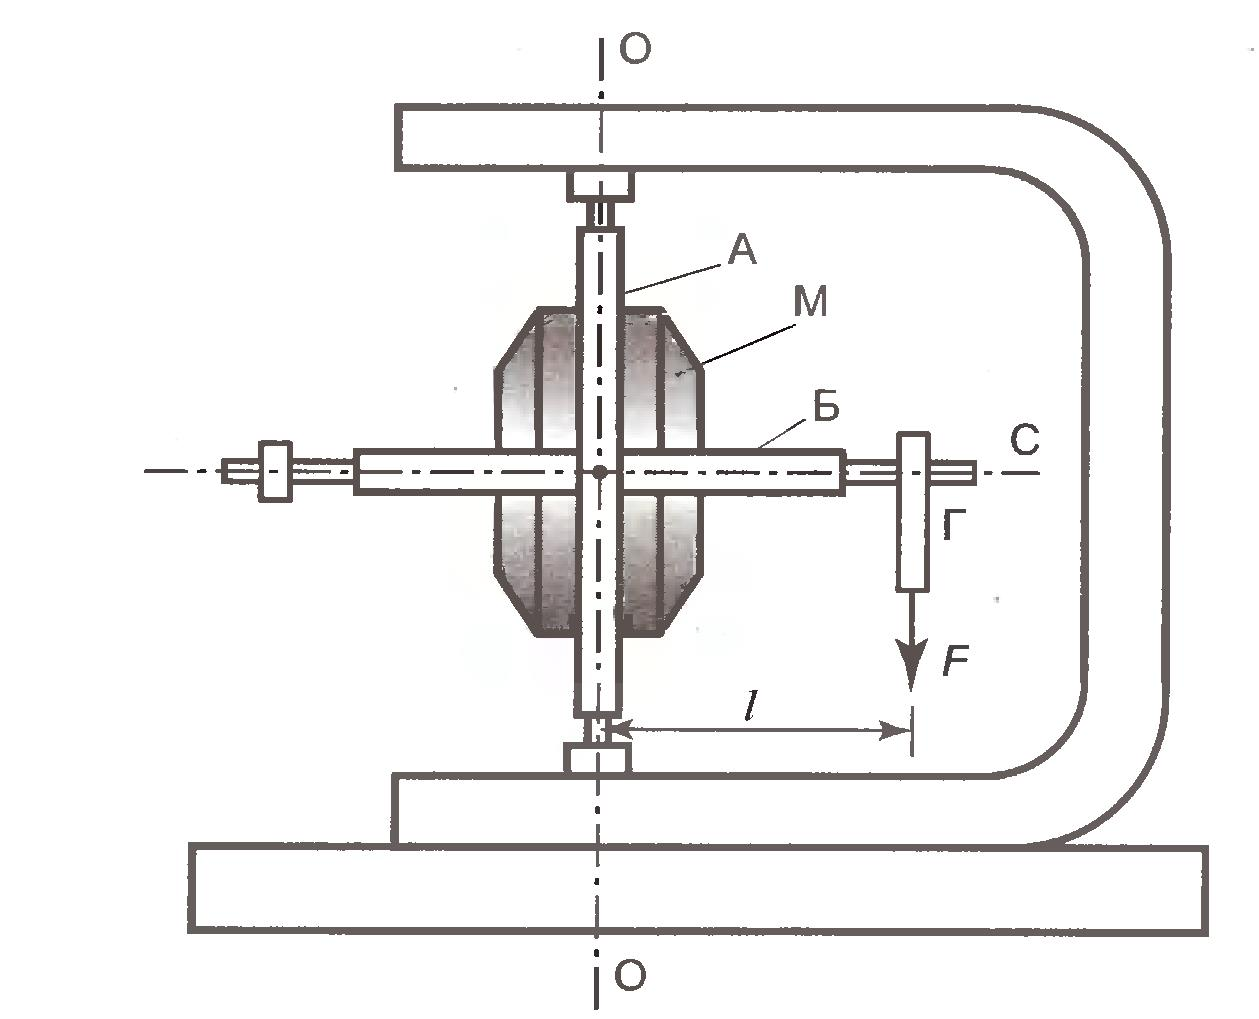
\includegraphics[width=0.45\linewidth]{facility} 
			\label{fig:facility} }  
	\caption{а) Гироскоп, закрепленный в карданном подвесе. б) Схема устройства гироскопа.}
\end{figure}

Ротором гироскопа (Рис. \ref{fig:facility}) является ротор электромотора М. Кожух мотора скреплен с кольцом Б (Рис. \ref{fig:Cardan_suspension}). Мотор с кольцом Б может вращаться в кольце А вокруг горизонтальной оси бб, которое может вращаться относительно оси аа. Рычаг С направлен по оси симметрии ротора. на рычаг подвешивают грузы Г.

Выше при выводе формул для прецессии предполагалось, что действующие на гироскоп силы лежат в плоскости $zy$, в которой лежат векторы угловых скоростей собственного вращения и прецессии. В этом случе, как уже говорилось, момент сил меняет лишь направление момента импульса гироскопа, но не его величину. Силу трения не лежат в плоскости осей вращения. Они приводят к измерению момента импульса и по направлению, и по величине. Для ротора гироскопа действие сил трения скомпенсировано действием электромотора. Для осей карданова подвеса компенсации нет. В результате ось гироскопа будет опускаться в направлении действия груза.

В первой части работы исследуется зависимость скорости прецесии гироскопа от момента силы, приложенной к его оси. Для этого к оси гироскопа (к рычагу $C$) подвешиваются грузы $\text{Г}$. Скорость прецессии определяется по числу оборотов рычага вокруг вертикальной оси и времени, которые на это ушло, определяемое секундомером. В процессе измерений рычаг не только поворачивается в результате прецессии гироскопа, но и опускается. Поэтому его в начале опыта следует приподнят на $5-6^{\circ}$. Опыт нао закончить, когда рычаг опустить на такой же угол.

Ихмерение скорости прецессии гироскопа позволяет вычислить угловую скорость вращения его ротора. Расчет производится по формуле (8). Момент инерции ротора относительно оси симметрии $I_0$ пизмеряется по крутильным колебаниям точной копии ротора, подвешиваемой вдоль оси симметриии наж есткой проволоке. Период крутильных колебаний $T_0$ зависит от момента инерции $I_0$ и модуля кручения проволоки $f$:
\[T_0 = 2\pi \sqrt{\frac{I_0}{f}}. \]

Чтобы исключить модуль кручения проволоки, вместо ротора гироскопа к той же проволоке подвешивабт цилиндр правильной форму с известным размерами и массов, для которого легко можно вычислить момент инерции $I_{\text{ц}}$. Для определения момента инерции ротора гироскопа имее \[ I_0 = I_{\text{ц}}\frac{T_0^2}{T_{\text{ц}}^2}, \]
здесь $I_{\text{ц}}$ -- период крутильным колебантй цилиндра.

Скорость вращения ротора гироскопа можно определить и не прибегая к исследованию прецессии. У используемых в работе гироскопов статор имеет две обмотки, необходимые для быстрой раскрутки гироскопа, а вторую -- для измерения числа оборотов ротора. Ротор электромотора всегда немного намагничен. Вращаясь, он наводит во второй обмотке переменную электродвижущую силу (ЭДС) индукции, частота которой равна частоте вращения ротора. Частоту этой ЭДС можно, в частности, измерить по фигурам Лиссажу, получаемым на экране осциллографа, если на вход подать исследуемую ЭДС, а на другой -- переменное напряжение с хорошо прокалиброванного генератор. При совпадении частот на экране получаем эллипс.



\begin{center}
\section{Выполнение работы.}
\end{center}

\subsection{Установка}
Устанавливаем ось гироскопа в горизонтальное положение, осторожно поворачивая ее за рычаг $C$.

\subsection{Включение питания}
Включаем питание гироскопа и ждем 4-5 минут, чтобы вращение ротора успело стабилизироваться.

\subsection{Вращение ротора}
Убеждаемся в том, что ротом вращается достаточно быстро: при легком постукивании по рычагу $C$ последний не должен изменят ьсвоего положения в пространтсве. <<Поиграемся>> с гироском, нажимая карандашом на рычаг $C$. По реакции гороскопа определяем в какую сторону вращается ротора.

\subsection{Прецессия гироскопа}
Подвесим к рычагу $C$ груз $\text{Г}$. При этом должна начаться прецессия гироскопа. Трение в оси приводит к тому, что рычаг $C$ начинает медленно опускаться.

\subsection{Измерение скорости прецесси $\Omega$}
Отклоняем рычаг $C$ на $5-6$ градусов вверх от горизонтальной плоскости. Подвесим к нему груз $\text{Г}$ и с помощью секундомера найдем угловую скорость регулярной прецесси $\Omega$, находить ее будем по числу оборотов и времени прецессии. Измерения продолжаем до тех пор, пока рычаг $C$  не опустится на $5-6$ градусов ниже горизонтальной плоскости, сделав целов число оборов относительно вертикальной оси. Измеряем также скорость опускания рычага $C$. Повторять опыт будем не менее пяти раз. В конце усредним результаты.
\begin{equation}
		T = \frac{t_{\text{полн}}}{N}
		\label{eq:period_equation}
	\end{equation}

\begin{equation}
	\Omega = \frac{2\pi n \pm \Delta\varphi}{t_{\text{полн}}}
	\label{eq:definition_Omega}
\end{equation} 
	

\subsection{Повторение прошлого пункта различных значениях момента $M$ силы $F$}
Проделаем всю серию экспериментов, описаннных в пункте 5 при $5-7$ значениях момента $M$ силы $F$ относительно центра масс гироскопа (длина плеча $l$ указана на установке). Результаты опытов изображаем в виде графика $\Omega$ в зависимости от $M$. 

\subsection{Измерение момента инерции ротора гироскопа}
Измеряем момент инерции ротора гироскопа относительно сои симметрии $I_0$. Для этого подвесим ротор, извлеченный из такого же гироскопа, к концу вертикально висящей проволоки так, чтобы ось симметрии гироскопа была вертикальна, и измеряем период крутильных колебаний получившегося маятника. Далее заменяем ротом гироскопа цилиндром, для которого известны или легко могут быть измерены радиус и масса, и определяем для него период крутильных колебаний. Пользуясь формулой (10) вычисляем момент инерции ротора гироскора $I_0$.

\begin{equation}
	I_{\text{ротора}}= I_{\text{ц}}\frac{T_{\text{ротора}}^2}{T_{\text{ц}}^2},
	\label{eq:moment_measuring_equation}
\end{equation}

\subsection{Погрешность}
Оцениваем погрешность в определении $I_0$ и $\Omega$ по следующим формулам:
\begin{equation}
	\varepsilon_{T} = \frac{\sigma_{T}}{T}
\end{equation}	

\begin{equation}
	\varepsilon_{I_{\text{ц}}} = \left(\frac{\sigma_{M}}{M}\right) + 2\left(\frac{\sigma_{R}}{R}\right)
\end{equation}	

\begin{equation}
	\varepsilon_{I_{0}} = \varepsilon_{I_{\text{ц}}} + \varepsilon_{T_{0}} + \varepsilon_{T_{\text{ц}}}
\end{equation}


\subsection{Частота вращения}
Рассчитаем с помощью (8) частоту вращения ротора гироскопа.

\subsection{Момент сил трения}
По скорости опускания рычага $C$ во время прецесии определяем момент сил трения.

\subsection{Фигуры Лиссажу}
Определим частоту вращения ротора гироскопа по фигурам Лиссажу. Для этого включаем осциллограф и генератор тумблерами <<Сеть>> и подаем на <<Вход $Y$>> осциллографа сигнал со второй обмотки статора гироскопа ( с двух клемм на подставке гиросокпа), а на <<Вход синхр.>> -- сигнал с выхода генератора. Для получения фигуры Лиссажу на осциллографе необходимо нажать тумблер <<Вход $X$>>, повернуть вправо до упора ручку <<Стабильность>>, переключателем <<Усилитель $U$>> добиваемся подходящего размера изображения по горизонтали. Переключателем <<Множитель частоты>> и рычкой <<$Hz$>> на генераторе добиваймся, чтобы на экране осциллографа появилась фигура, похожая на эллипс.  Подбираем частоту генератора так, чтобы эллипс стал неподвижным. Если этого сделать не удается, то выключаем на короткое время питание электромотора гироскопа, чтобы ток первый обмотки не наводил ЭДС во второй и не мешал измерениям. Делать измерения при этом надо быстро, так как при выключенном питании ротор гироскопа начинает замедлять свое вращения. Получение на экране осциллографа неподвижного эллипса означает, что частота сигнала генератора равна частоте вращения ротора гироскопа.

\subsection{Погрешность полученных результатов}
Оценим погрешность полученных результатов. Сравним угловые скорости вращения ротора гироскопа, определяемые разными методами. Погрешность частоты вращения ротора по фигурам Лиссажу будем находить по МНК.

\begin{equation}
	\sigma_{M} = \sqrt{\varepsilon_{\alpha}^{2} + \varepsilon_{I_{0}}^{2} + \varepsilon_{\omega_{z}}^{2} + \varepsilon_{t_{\text{полн}}}^{2}}
\end{equation}

\begin{equation}
	\sigma_{\alpha} = \frac{\partial \alpha}{\partial \frac{\Delta h}{l}} = \frac{\sigma_{\frac{\Delta h}{l}}}{1 + \frac{\Delta h}{l}}
\end{equation}

\begin{center}
\section{Результаты}
\end{center}

\begin{enumerate}
	\item В ходе выполнения работы были определены физические величины, описывающие регулярную прецессию гироскопа, закрепленного в карданном подвесе, а именно:
		\begin{itemize}
			\item Была определена теоретически и экспериментально угловая скорость регулярной прецессии гироскопа. Полученная точность теоретически определенной величины совпадает с точностью, с которой можно определить момент инерции ротора гироскопа, так как эта величина вносит наибольший вклад в погрешность.
			\item Был определен момент инерции ротора гироскопа.Основной вклад -- погрешность измерения радиуса цилиндра, с помощью которого определялась данная величина.
			\item Был определен момент сил трения, возникающих в оси карданного подвеса. Основной вклад: погрешность измерения угла отклонения оси от горизонтальной плоскости, погрешность фиксирования прохождения оси через начальную точку.
		\end{itemize}
	\item На практике были подтверждены все теоретические зависимости, используемые в данной работе.
	\item Показано соответствие различных методов определения физических величин : угловая скорость, частота.
	\item Достигнута приемлемая точность.
\end{enumerate}



\end{document}


